\section{Electromagnetic induction}

\begin{Exercise}[difficulty=2]
The triangular frame is rotating with angular velocity ($\omega$) in homogeneous, steady magnetic field $\vec B$. Calculate electromotive force induced in the frame.
\begin{center}
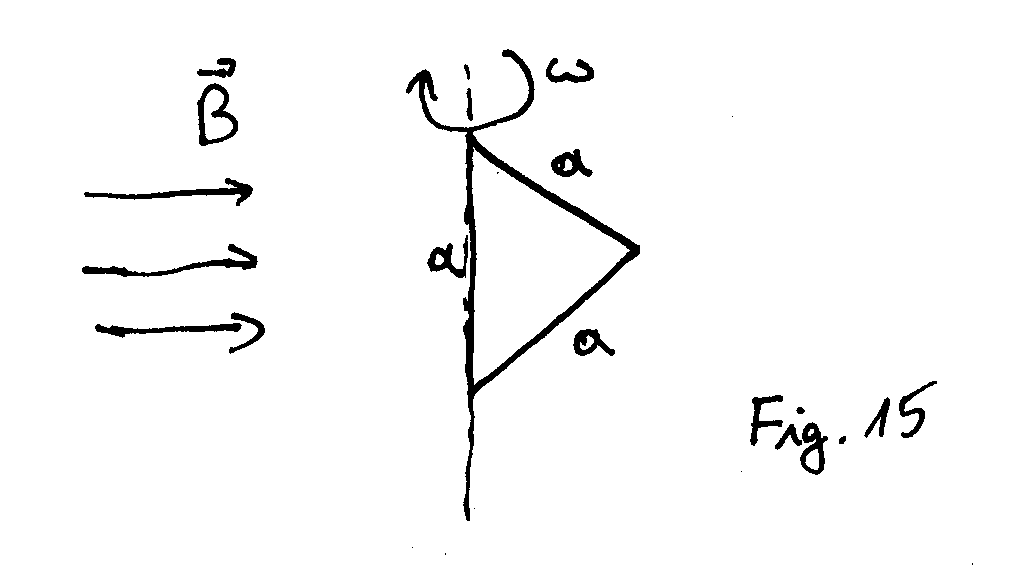
\includegraphics[width=0.4\textwidth]{img/fig_ind1.png} 
\end{center}
\end{Exercise}

\begin{Exercise}[difficulty=2]
The conducting bar is sliding on u-shaped frame made of metal, int the presence of homogeneous, steady magnetic field $\vec B$. Find equation describing current flowing in the circuit. Assume that resistivity of conductors and dimensions of object are given.
\begin{center}
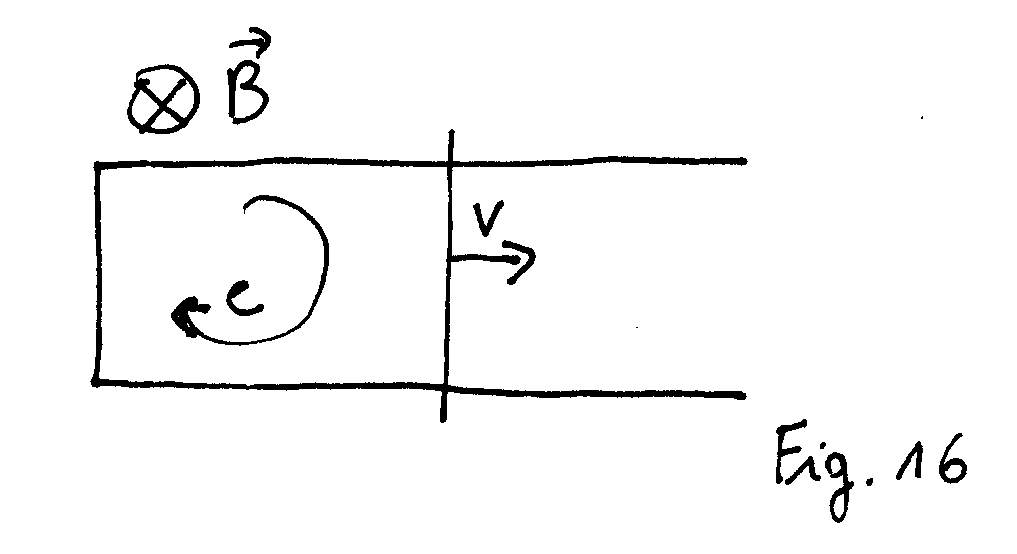
\includegraphics[width=0.4\textwidth]{img/fig_ind2.png} 
\end{center}
\end{Exercise}

\begin{Exercise}[difficulty=3]
Alternating current (AC) flows in the straight line cable with magnitude $I_1$ and angular velocity $\omega$. What is the electromotive force induced in the rectangular frame ($b$ by $c$) located in the distance $a$ from the cable?
\begin{center}
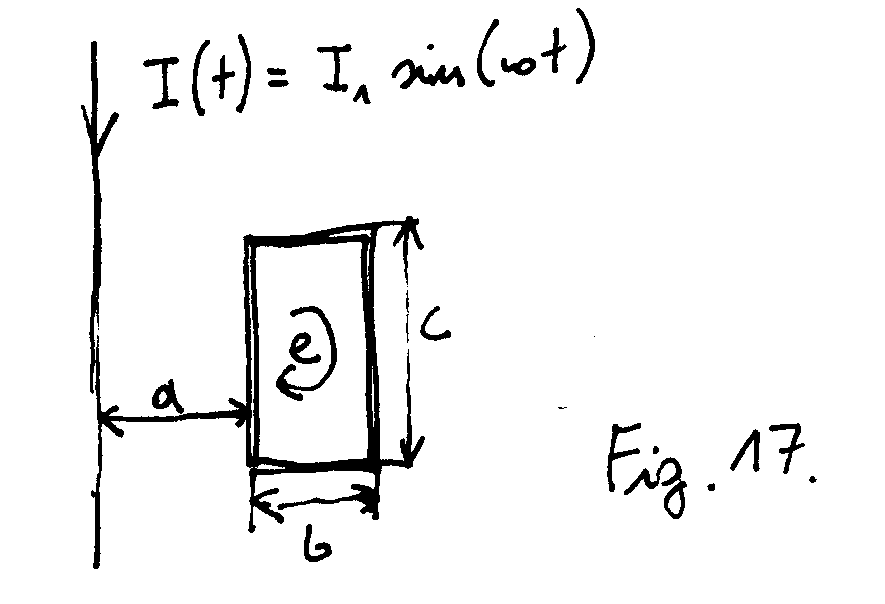
\includegraphics[width=0.4\textwidth]{img/fig_ind3.png} 
\end{center}
\end{Exercise}

